\documentclass[margin=0px]{article}

\usepackage{listings}
\usepackage[utf8]{inputenc}
\usepackage{graphicx}
\usepackage{float}
\usepackage[a4paper, margin=0.7in]{geometry}
\usepackage{amsthm}
\usepackage{amssymb}
\usepackage{t1enc}
\usepackage{fancyhdr}
\usepackage{setspace}

\onehalfspacing

\newenvironment{tetel}[1]{\paragraph{#1 \\}}{}

\pagestyle{fancy}
\lhead{\it{PTI BSc Záróvizsga tételek}}
\rhead{17. Operációs rendszerek}

\title{\textbf{{\Large ELTE IK - Programtervező Informatikus BSc} \vspace{0.2cm} \\ {\huge Záróvizsga tételek}} \vspace{0.3cm} \\ 17. Operációs rendszerek}
\author{}
\date{}

\begin{document}
\maketitle

\begin{tetel}{Operációs rendszerek}
    Folyamatok megvalósítása, ütemező algoritmusaik. Párhuzamosság, kritikus szekciók, kölcsönös kizárás megvalósítása. Peterson algoritmus. Szemaforok, osztott memória, üzenetküldés. Be-és kimeneti eszközök ütemezési lehetőségei, holtpontok. Memóriakezelés, virtuális memóriakezelés fogalma. Lapozás és szegmentálás. Lapcserélési algoritmusok (pl: LRU). Háttértárak, redundancia, fájlrendszerek, alapvető típusaik és szolgáltatásaik, jellemzőik.
\end{tetel}

\section{Operációs rendszer}
Olyan programrendszer, amely a számítógépes rendszerben a programok végrehajtását vezérli: így például ütemezi a programok végrehajtását, elosztja az erőforrásokat, biztosítja a felhasználó és a számítógépes rendszer közötti kommunikációt. Olyan program, ami egyszerű felhasználói felületet nyújt, eltakarva a számítógép(rendszer) eszközeit. \\

\section{Folyamatok megvalósítása, ütemező algoritmusaik}

\subsection{Folyamatok megvalósítása}

\textit{Program}: fájlrendszerben egy bájthalmaz. \\
\textit{Folyamat}(processz): futó program a memóriában (kód + I/O adatok + állapot). \\
Egyszerre hány folyamat működik? \\
Valódi multitask esetén egymástól teljesen függetlenül mennek a folyamatok. Operációs rendszerek egy szekvenciális modellt követnek, ami álmultitasking. Itt egyidejűleg a memóriához csak egy folyamat fér hozzá, gyorsan váltogat a dolgok között (multiprogramozás). \\
Az operációs rendszernek ahhoz, hogy ezeket a folyamatokat helyesen tudja kezelni, felügyelnie kell a folyamatokat. Az operációs rendszerünk így minden egyes folyamatot nyilvántart, és az operációs rendszer lelkének is nevezett ütemező (scheduler) segítségével szépen sorban minden egyes folyamatnak ad egy kis processzor- (CPU) időszeletet, amíg az adott folyamat dolgozik, azaz a processzorra kerülhet.
\textit{Rendszer modell}: 1 processzor + 1 rendszer memória + 1 I/O eszköz = 1 feladat-végrehajtás \\
Interaktív (ablakos) rendszerekben több program, processz fut.
\begin{itemize}
    \item Környezetváltásos rendszer: csak az előtérben lévő alkalmazás fut
    \item Kooperatív rendszer: az aktuális processz bizonyos időközönként, vagy időkritikus műveletnél önként lemond a CPU-ról (Win 3.1)
    \item Preemptív rendszer: az aktuális processztől a kernel bizonyos idő után elveszi a vezérlést, és a következő várakozó folyamatnak adja.
    \item Real time rendszer: egy operációs rendszer nyújtson lehetőséget az időfaktor figyelembe vételéhez. A mai OR-ek kezdenek ilyen tulajdonságokkal is kiegészülni.
\end{itemize}

\textit{Folyamatok létrehozása}: ma tipikusan preemptív rendszereket használunk. Létrehozás oka lehet: rendszer inicializálás, folyamatot eredményező rendszerhívás (másolat az eredetiről [fork], az eredeti cseréje [execve]), felhasználói kérés (parancs\&), nagy rendszerek kötegelt feladatai. \\
A folyamatok futhatnak az előtérben, illetve a háttérben. Ez utóbbiakat hívjuk démonoknak.\\
\textit{Folyamatok kapcsolata}: Szülő-gyermek kapcsolat, folyamatfa: egy folyamatnak egy szülője van, egy folyamatnak viszont lehet több gyereke is, vannak összetartozó folyamatcsoportok. \\ Reinkarnációs szerver: meghajtó programok, kiszolgálók elindítója, ha elhal az egyik, akkor azt újraszüli, reinkarnálja. \\
\textit{Folyamatok befejezése}: Egy folyamat az elindulása után a megadott időkeretben (el)végzi a feladatát. A befejezés lehet önkéntes vagy önkéntelen.
\begin{itemize}
    \item Önkéntes befejezések: Szabályos kilépés (exit, return stb.), Kilépés valamilyen hiba miatt, amit a program felfedez (szintén pl. return utasítással).
    \item Önkéntelen befejezések: Illegális utasítás, végzetes hiba (0-val osztás, nem létező memória használat, stb), Külső segítséggel: Másik processz, netán mi ,,lőjük” ki az adott folyamatot.
\end{itemize}
\textit{Folyamatok állapota}: A folyamat önálló programegység, saját utasításszámlálóval, veremmel stb. Általában nem függetlenek a folyamatok, egyik-másik eredményétől függ a tevékenység. Egy folyamat három állapotban lehet:
\begin{itemize}
    \item Futó
    \item Futásra kész, ideiglenesen leállították, arra vár, hogy az ütemező CPU időt adjon a folyamatnak
    \item Blokkolt, ha logikailag nem lehet folytatni a tevékenységet, mert pl. egy másik eredményére vár. (catFradi.txt|grepFradi|sort, grep és sort blokkolt az elején)
\end{itemize}
\begin{figure}[H]
    \centering
    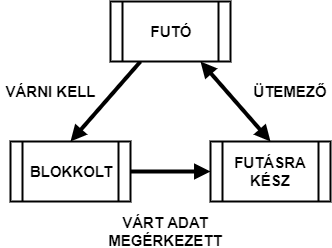
\includegraphics[width=0.6\textwidth]{img/allapot.png}
    \caption{Állapotátmenetek}
\end{figure}

\textit{További állapotok}: alvó, megállított, zombi (ha egy gyermek folyamat befejeződik, de szülője nem hív wait(\&st) hívást, akkor a gyermek bent marad a processztáblában, init folyamat törli ezeket). \\
\textit{\textbf{Folyamatok megvalósítása}}: A processzor csak végrehajtja az aktuális utasításokat. Egyszerre egy folyamat aktív. Folyamatokról nem tud a processzor. Ha lecseréljük az aktív folyamatot a következőre, akkor mindent meg kell őrizni, hogy visszatérhessünk a folytatáshoz. A ,,minden": utasításszámláló, regiszterek, lefoglalt memória állapot, nyitott fájl infók, stb. Ezeket az adatokat az úgynevezett folyamatleíró táblában tároljuk (processz tábla, processz vezérlő blokk). Van egy I/O megszakításvektor is. \\
A folyamatokat úgy is osztályozhatjuk, hogy számításigényes vagy input/output-igényes (avagy beviteli/kiviteli, röviden B/K vagy I/O) folyamatról van-e szó. Könnyen belátható, hogy a számításigényes folyamatoknak az a legjobb, ha az ütemező általában hosszú időperiódusra adja meg nekik a processzort, míg az input/output-igényes folyamatoknak a rövidebb periódusidő a megfelelőbb.

\subsection{Ütemező algoritmusok}

\textit{Folyamatok váltása}: Kezdeményezheti időzítő, megszakítás, esemény, rendszerhívás kezdeményezés. Az ütemező elmenti az aktuális folyamat jellemzőket a folyamatleíró táblába. Betölti a következő folyamat állapotát, a processzor folytatja a munkát. Nem lehet menteni a gyorsítótárakat. Gyakori váltás többleterőforrást igényel. A folyamatváltási idő „jó” megadása nem egyértelmű. \\
\textit{Folyamatleíró táblázat}(Process Control Block - PCB): A rendszer inicializálásakor létrejön; 1 elem, rendszerindító már bent van, mikor a rendszer elindul. Tömbszerű szerkezet (PID alapon), de egy-egy elem egy összetett processzus adatokat tartalmazó struktúra. Egy folyamat fontosabb adatai: Azonosítója (ID), neve (programnév); Tulajdonos, csoport azonosító; Memória, regiszter adatok stb. \\
\textit{Szálak}: Önállóan működő programegységek (thread), egy folyamaton belüli különálló utasítássor. Általában egy folyamat = egy utasítássorozat = egy szál. Néha szükséges lehet, hogy egy folyamaton belül ,,több utasítássorozat" legyen. Gyakran ,,lightweight process"-nek nevezik a több utasítássorozatos folyamatot. Egy folyamaton belül több egymástól ,,független" végrehajtási sor lehet. Lehet egy folyamaton belül egy szál vagy egy folyamaton belül több szál. Ez utóbbi esetben, ha egy szál blokkolódik, a folyamat is blokkolva lesz. Van külön száltáblázat. \\
Folyamatnak önálló címtartománya van, globális változói, megnyitott fájlleírói, gyermekfolyamatai, szignálkezelői, ébresztői stb., szálnak ezek nincsenek; viszont mindkettőnek vannak utasításszámlálói, regiszterei, van verme. \\ \\

Egyszerre csak 1 folyamat tud futni. Az ütemező hozza meg a döntést. Ütemezési algoritmus alapján dönti el, hogy melyik fusson. \\
Folyamatváltás biztosan van: ha befejeződik egy folyamat, vagy ha egy folyamat blokkolt állapotba kerül (I/O vagy szemafor miatt). Általában van váltás: ha új folyamat jön létre, I/O megszakítás bekövetkezés (I/O megszakítás után jellemzően egy blokkolt folyamat, ami erre várt, folytathatja futását), időzítő megszakítás (nem megszakítható ütemezés, megszakítható ütemezés). \\
Ütemezések csoportosítása:
\begin{itemize}
    \item Minden rendszerre jellemző a pártatlanság, hogy mindenki hozzáférhet a CPU-hoz, ugyanazok az elvek érvényesek mindenkire, és ,,azonos” terhelést kapnak.
    \item Kötegelt rendszerek: Áteresztőképesség, áthaladási idő, CPU kihasználtság
    \item Interaktív rendszerek: Válaszidő, megfelelés a felhasználói igényeknek
    \item Valós idejű rendszerek: Határidők betartása, adatvesztés, minőségromlás
          elkerülése
\end{itemize}
\textbf{Ütemezés kötegelt rendszerekben}:
\begin{itemize}
    \item Sorrendi ütemezés, nem megszakítható
          \begin{itemize}
              \item First Come First Served - (FCFS)
              \item Egy folyamat addig fut, amíg nem végez, vagy nem blokkolódik.
              \item Ha blokkolódik, a sor végére kerül.
              \item Pártatlan, egyszerű, láncolt listában tartjuk a folyamatokat.
              \item Hátránya: I/O igényes folyamatok nagyon lassan végeznek.
          \end{itemize}
    \item Legrövidebb feladat először, nem megszakítható ez se (shortest job first -- SJB)
          \begin{itemize}
              \item Kell előre ismerni a futási időket
              \item Akkor optimális, ha kezdetben mindenki elérhető
          \end{itemize}
    \item Legrövidebb maradék futási idejű következzen
          \begin{itemize}
              \item Megszakítható, minden új belépéskor vizsgálat.
          \end{itemize}
    \item Háromszintű ütemezés
          \begin{itemize}
              \item Bebocsátó ütemező: A feladatokat válogatva engedi be a memóriába.
              \item Lemez ütemező: Ha a bebocsátó sok folyamatot enged be és elfogy a memória, akkor lemezre kell írni valamennyit, meg vissza. Ez ritkán fut.
              \item CPU ütemező: A korábban említett algoritmusok közül választhatunk.
          \end{itemize}
\end{itemize}
\textbf{Ütemezés interaktív rendszerekben}:
\begin{itemize}
    \item Körben járó ütemezés -- Round Robin
          \begin{itemize}
              \item Mindenkinek időszelet, aminek végén, vagy blokkolás esetén jön a következő folyamat
              \item Időszelet végén a körkörös listában következő lesz az aktuális folyamat
              \item Pártatlan, egyszerű
              \item Egy listában tárolhatjuk a folyamatokat (jellemzőit), és ezen megyünk körbe-körbe.
              \item Időszelet mérete lehet probléma, mert a processz átkapcsolás időigényes. Ha kicsi az idő, akkor sok CPU megy el a kapcsolgatásra, ha pedig túl nagy, akkor interaktív felhasználóknak lassúnak tűnhet pl a billentyűkezelés.
          \end{itemize}
    \item Prioritásos ütemezés
          \begin{itemize}
              \item Fontosság, prioritás bevezetése. Unix: 0-49 nem megszakítható (kernel) prioritás, 50-127 user prioritás
              \item Legmagasabb prioritású futhat. Dinamikus prioritás módosítás, különben éhenhalás
              \item Prioritási osztályok használata. Egy osztályon belül Round Robin. Ki kell igazítani a folyamatok prioritását, különben az alacsonyak nagyon ritkán jutnak CPU-hoz. Tipikusan minden 100 időszeletnél a prioritásokat újraértékeli és ilyenkor jellemzően a magas prioritások alacsonyabbra kerülnek, majd ezen a soron megy RR. A végén újra felállnak az eredeti osztályok.
          \end{itemize}
    \item Többszörös sorok
          \begin{itemize}
              \item Szintén prioritásos és RR
              \item Legmagasabb szinten minden folyamat 1 időszeletet kap
              \item Következő 2-t, majd 4-et, 8, 16,32,64-et.
              \item Ha elhasználta a legmagasabb szintű folyamat az idejét egy szinttel lejjebb kerül.
          \end{itemize}
    \item Legrövidebb folyamat előbb
          \begin{itemize}
              \item Bár nem tudjuk a hátralévő időt, de becsüljük meg az előzőekből.
              \item Öregedés, súlyozott átlag az időszeletre: T0, T0/2+T1/2, T0/4+T1/4+T2/2, T0/8+T1/8+T2/4+T3/2
          \end{itemize}
    \item Garantált ütemezés
          \begin{itemize}
              \item Minden aktív folyamat arányos CPU időt kap.
              \item Nyilván kell tartani, hogy egy folyamat már mennyi időt kapott, ha valaki arányosan kevesebb időt kapott, az kerül előbbre.
          \end{itemize}
    \item Sorsjáték ütemezés
          \begin{itemize}
              \item Mint az előző, csak a folyamatok között ,,sorsjegyeket" osztunk szét, az kapja a vezérlést, akinél a kihúzott jegy van
              \item Arányos CPU időt könnyű biztosítani, hasznos pl. video szervereknél
          \end{itemize}
    \item Arányos ütemezés
          \begin{itemize}
              \item Vegyük figyelembe a felhasználókat is. Olyan, mint a garantált, csak a felhasználókra vonatkoztatva.
          \end{itemize}
\end{itemize}
\textbf{Ütemezés valós idejű rendszerekben} \\
A valós idejű rendszerben az idő kulcsszereplő. Garantálni kell adott határidőre a tevékenység, válasz megadását.
\begin{itemize}
    \item Hard Real Time (szigorú), abszolút, nem módosíthatóhatáridők.
    \item Soft Real Time (toleráns), léteznek a határidők, de ezek kis mértékű elmulasztása tolerálható.
\end{itemize}
A programokat több kisebb folyamatra bontják. Külső esemény észlelésekor, adott határidőre válasz
kell. Ütemezhető: ha egységnyi időre eső n esemény CPU válaszidő összege <=1. \\
Gyakori a gyermek folyamatok jelenléte a rendszerben. A szülőnek nem biztos, hogy minden
gyermekével azonos prioritásra van szüksége. Tipikusan a kernel \textit{prioritásos ütemezést}
használ (+RR):
\begin{itemize}
    \item Biztosít egy rendszerhívást, amivel a szülő a gyermek prioritását adhatja meg
    \item Kernel ütemez -- felhasználói folyamat szabja meg az elvet, prioritást.
\end{itemize}

\textbf{Szálütemezés}:
\begin{itemize}
    \item Felhasználói szintű szálak
          \begin{itemize}
              \item Kernel nem tud róluk, a folyamat kap időszeletet, ezen belül a szálütemező dönt ki fusson
              \item Gyors váltás a szálak között
              \item Alkalmazásfüggő szálütemezés lehetséges
          \end{itemize}
    \item Kernel szintű szálak
          \begin{itemize}
              \item Kernel ismeri a szálakat, kernel dönt melyik folyamat melyik szála következzen
              \item Lassú váltás, két szál váltása között teljes környezetátkapcsolás kell
              \item Ezt figyelembe is veszik.
          \end{itemize}
\end{itemize}

\section{Párhuzamosság, kritikus szekciók, kölcsönös kizárás megvalósítása}

\subsection{Párhuzamosság és megvalósítása}

Ütemező a folyamatok gyors váltogatásával ,,teremt" párhuzamos végrehajtás érzetet. \\
Többprocesszoros rendszerekben több processzor van egy gépben, nagyobb a teljesítmény, de a megbízhatóságot általában nem növeli. \\
Klaszterek: megbízhatóság növelése elsősorban a cél.

\subsection{Kritikus szekciók}

Azokat az utasításokat, azt a programrészt, amelyben a programunk a közös adatokat használja, kritikus területnek, kritikus szekciónak vagy kritikus blokknak nevezzük. \\
Kulcskérdés: a közös erőforrások használata, amikor két folyamat ugyanazt a memóriát használja. Kritikus programterület, szekció, az a rész, mikor a közös erőforrást (memóriát) használjuk. \\
Versenyhelyzet: két vagy több folyamat közös memóriát ír vagy olvas, a végeredmény a futási időpillanattól függ. Nehezen felderíthető hibát okoz. \\
Megoldás: Módszer, ami biztosítja, hogy a közös adatokat egyszerre csak egy folyamat tudja használni.

\subsection{Kölcsönös kizárás és megvalósítása}

Kölcsönös kizárásnak nevezzük azt a módszert, ami biztosítja, hogy ha egy folyamat használ valamilyen megosztott, közös adatot, akkor más folyamatok ebben az időben ne tudják azt elérni. \\
A jó kölcsönös kizárás az alábbi feltételeknek felel meg:
\begin{itemize}
    \item Nincs két folyamat egyszerre a kritikus szekciójában.
    \item Nincs sebesség, CPU paraméter függőség.
    \item Egyetlen kritikus szekción kívül levő folyamat sem blokkolhat másik folyamatot.
    \item Egy folyamat sem vár örökké, hogy a kritikus szekcióba tudjon belépni.
\end{itemize}

\begin{figure}[H]
    \centering
    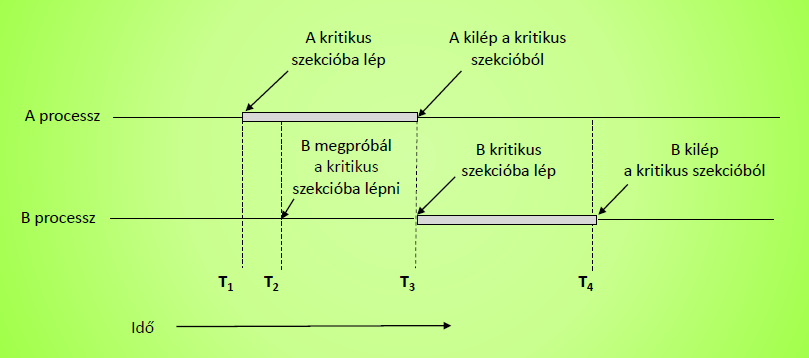
\includegraphics[width=0.9\textwidth]{img/mutex.png}
    \caption{A megkívánt kölcsönös kizárás viselkedése}
\end{figure}

\subsubsection{Megvalósítások}

\begin{itemize}
    \item Megszakítások tiltása (összes): Belépéskor az összes megszakítás tiltása, Kilépéskor azok engedélyezése. Ez nem igazán jó, mivel a felhasználói folyamatok kezében lenne a megszakítások tiltása, persze a kernel használja.
    \item Osztott, ún. zárolás változó használata: 0 (senki) és 1 (valaki) kritikus szekcióban van. Két folyamat is kritikus szekcióba tud kerülni! Egyik folyamat belép a kritikus szekcióba, de éppen az 1-re állítás előtt a másik folyamat kerül ütemezésre.
    \item Szigorú váltogatás: Több folyamatra is általánosítható. A kölcsönös kizárás feltételeit teljesíti a 3. kivételével, ugyanis ha pl 1 folyamat a lassú, nem kritikus szekcióban van, és a 0 folyamat gyorsan belép a kritikus szekcióba, majd befejezi a nem kritikus szekciót is, akkor ez a folyamat blokkolódik mert a kovetkezo=1 lesz!(Saját magát blokkolja!)
          \begin{figure}[H]
              \centering
              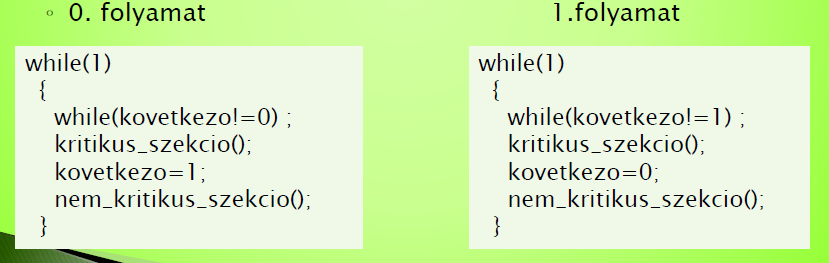
\includegraphics[width=0.9\textwidth]{img/szigoru.png}
              \caption{Szigorú váltogatás}
          \end{figure}
    \item G. L. Peterson javította a szigorú váltogatást. A kritikus szekció előtt minden folyamat meghívja a belépés, majd utána kilépés függvényt.
          \begin{figure}[H]
              \centering
              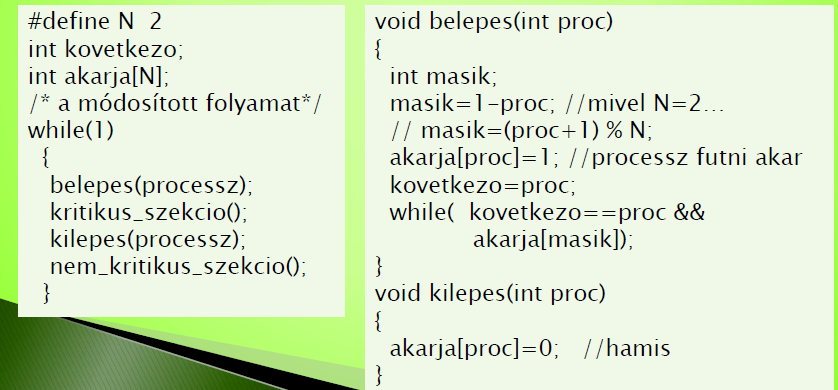
\includegraphics[width=0.6\textwidth]{img/peterson.png}
              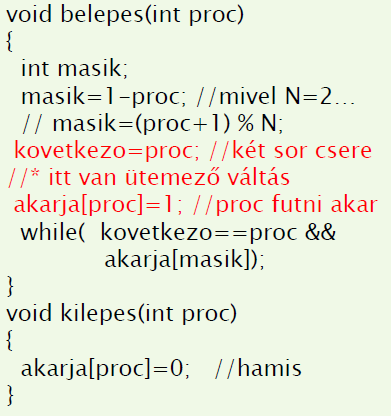
\includegraphics[width=0.3\textwidth]{img/petersonhiba.png}
              \caption{Peterson javítása és a benne rejlő hiba}
          \end{figure}
          Ez a javítás viszont nagy hibát okozhat. Tegyük fel proc=0. A jelölt ütemezés váltásnál a proc=1 belépése jön. Mivel akarja[0] értéke 0, ezért az 1-es process belép a kritikus szakaszba! Ekkor újra váltson az ütemező, akarja[1]=1, a következő értéke szintén 1, így a következo==proc hamis, azaz a 0. proc is belép a kritikus szakaszba!
    \item Tevékeny várakozás gépi kódban: TSL utasítás, Test and Set Lock. Ez atomi művelet, vagyis megszakíthatatlan.
    \item Tevékeny várakozás: A korábbi Peterson megoldás is, a TSL használata is jó, csak ciklusban várakozunk. A korábbi megoldásokat, tevékeny várakozással (aktív várakozás) megoldottnak hívjuk, mert a CPU-t ,,üres" ciklusban járatjuk a várakozás során.De ez a CPU időt pazarolja. Helyette jobb lenne az, ha a kritikus szekcióba lépéskor blokkolna a folyamat, ha nem szabad belépnie. Az aktív várakozás nem igazán hatékony. Megoldás: blokkoljuk(alvás) várakozás helyett a folyamatot, majd ha megengedett ébresszük fel. Különböző paraméter megadással is implementálhatók. Tipikus probléma: Gyártó-Fogyasztó probléma vagy másképp korlátos tároló probléma. PL: Pék-pékség-Vásárló háromszög:
          \begin{itemize}
              \item A pék süti a kenyeret, amíg a pékség polcain van hely.
              \item Vásárló tud venni, ha a pékség polcain van kenyér.
              \item Ha tele van kenyérrel a pékség, akkor ,,a pék elmegy pihenni".
              \item Ha üres a pékség, akkor a vásárló várakozik a kenyérre.
          \end{itemize}
          \begin{figure}[H]
              \centering
              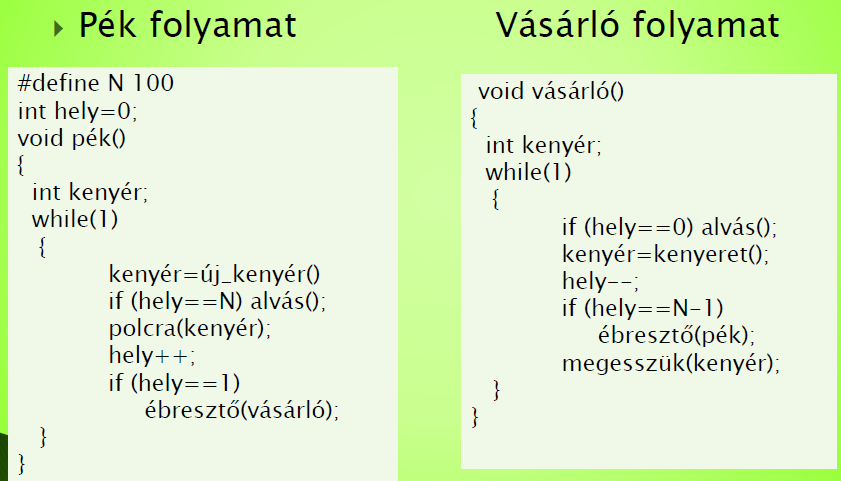
\includegraphics[width=0.9\textwidth]{img/pekvasarlo.png}
              \caption{Gyártó-fogyasztó probléma egy megvalósítása}
          \end{figure}
          Ennél a megvalósításnál probléma lehet, hogy A ,,hely" változó elérése nem korlátozott, így ez okozhat versenyhelyzetet.
          \begin{itemize}
              \item Vásárló látja, hogy a hely 0 és ekkor az ütemező átadja a vezérlést a péknek, aki süt egy kenyeret. Majd látja, hogy a hely 1, ébresztőt küld a vásárlónak. Ez elveszik, mert még a vásárló nem alszik.
              \item Vásárló visszakapja az ütemezést, a helyet korábban beolvasta, az 0, megy aludni.
              \item A pék az első után megsüti a maradék N-1 kenyeret és ő is aludni megy
          \end{itemize}
          Lehet ébresztő bittel javítani, de több folyamatnál a probléma nem változik.
\end{itemize}

\section{Szemaforok, osztott memória, üzenetküldés}

\subsection{Szemaforok}

E.W. Dijkstra(1965) javasolta ezen új változótípus bevezetését.
\begin{itemize}
    \item Ez valójában egy egész változó.
    \item A szemafor tilosat mutat, ha értéke 0. Ekkor a folyamat elalszik, megáll a tilos jelzés előtt.
    \item Ha a szemafor >0, szabad a pálya, beléphetünk a kritikus szakaszra. Két művelet tartozik hozzá: ha beléptünk, csökkentjük szemafor értékét (down); ha kilépünk, növeljük a szemafor értékét (up). Ezeket Dijkstra P és V műveletnek nevezte.
\end{itemize}
Elemi művelet: a szemafor változó ellenőrzése, módosítása, esetleges elalvás oszthatatlan művelet, nem lehet megszakítani. Ez garantálja, hogy ne alakuljon ki versenyhelyzet. \\
Ha a szemafor tipikus vasutas helyzetet jelöl, azaz 1 vonat mehet át csak a jelzőn, a szemafor értéke ekkor 0 vagy 1 lehet. Ez a \textit{bináris szemafor}, vagy más néven MUTEX (Mutual Exclusion), és kölcsönös kizárásra használjuk. \\
Rendszerhívással, felhasználói szinten nem biztosítható a műveletek atomiságának megvalósítása. Művelet elején például letiltunk minden megszakítást. Ha több CPU van, akkor az ilyen szemafort védeni tudjuk a TSL utasítással. Viszont ezek a szemafor műveletek kernel szintű, rendszerhívás műveletek. A fejlesztői környezetek biztosítják.
\begin{figure}[H]
    \centering
    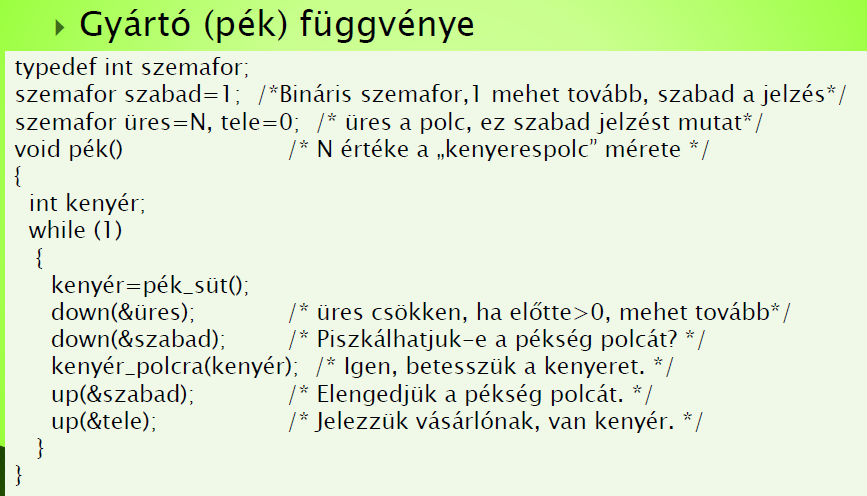
\includegraphics[width=0.45\textwidth]{img/gyarto_szemafor.png}
    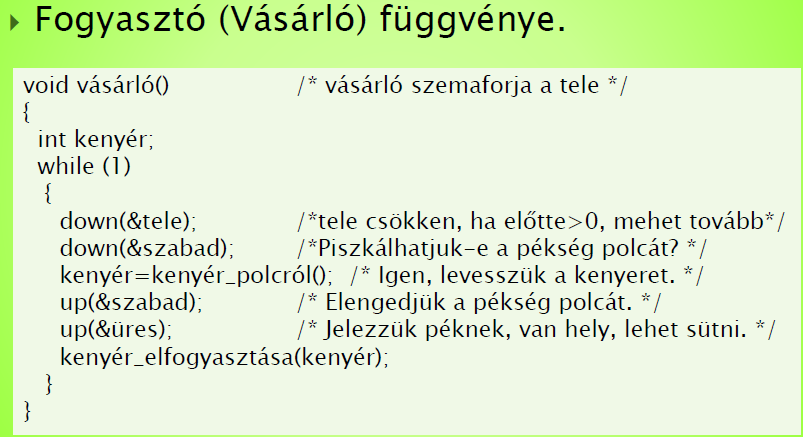
\includegraphics[width=0.45\textwidth]{img/fogyaszto_szemafor.png}
    \caption{Gyártó-fogyasztó probléma megoldása szemaforokkal}
\end{figure}
\textit{Szabad}: kenyér polcot (boltot) védi, hogy egy időben csak egy folyamat tudja használni (vagy a pék, vagy a vásárló): Kölcsönös kizárás, Elemi műveletek (up, down). \\
\textit{Tele, üres szemafor}: szinkronizációs szemaforok, a gyártó álljon meg ha a tároló tele van, illetve a fogyasztó is várjon ha a tároló üres. \\ \\
Szemafornál két utasítás felcserélése is gondot okozhat. \\
\textit{Monitor}: magasabb szintű, nyelvű konstrukció. Eljárások, adatszerkezetek
lehetnek benne. Egy időben csak egy folyamat lehet aktív a monitoron belül.

\subsection{Osztott memória}

Elosztott közös memória: Hálózatban futó folyamatok közti memóriamegosztás. \\
Lehetőségünk van egy programon belüli különböző folyamatok, szálak által használt memóriaterületek közössé tételére, vagyis használhatjuk ugyanazt a memóriarészt, ,,időosztásos" üzemmódban. Különböző, egymással valamilyen módon ,,összekapcsolt" programrészekhez, folyamokhoz, szálakhoz ugyanazt a memóriaterület kapcsoljuk.

\subsection{Üzenetküldés}

A folyamatok jellemzően két primitívet használnak: \textit{Send(célfolyamat, üzenet)}, \textit{Receive(forrás, üzenet)}. Ezek rendszerhívások, nem nyelvi konstrukciók. \\
Ha küldő-fogadó nem azonos gépen van, szükséges ún. nyugtázó üzenet. Így ha küldő nem kapja meg a nyugtát, ismét elküldi az üzenetet. Ha a nyugta veszik el, a küldő újra küld. Ismételt üzenetek megkülönböztetése sorszám segítségével történik. \\
\textit{Összegzés}: Ideiglenes tároló helyek (levelesláda) létrehozása mindkét helyen. El lehet hagyni, ekkor ha send előtt van receive, a küldő blokkolódik, illetve fordítva. Ezt hívják randevú stratégiának. Például a  Minix 3 is randevút használ, rögzített méretű üzenetekkel. \\
Adatcső kommunikáció hasonló, csak az adatcsőben nincsenek üzenethatárok, ott csak bájtsorozat van. Az üzenetküldés a párhuzamos rendszerek általános technikája. Pl. MPI \\
Klasszikus IPC (inter-process communication) problémák:
\begin{itemize}
    \item Étkező filozófusok esete: körben felváltva 5 villa, tányér. 2 villa kell a spagetti
          evéshez. A tányér melletti villákra pályáznak. Esznek-gondolkoznak. A legegyszerűbb megoldás (végtelen ciklusban gondolkodik, felveszi a két villáját egymás után, eszik, leteszi a villákat) pár hibát rejt magában, hogy pl. holtpont lehet, ha egyszerre megszerzik a bal villát és mind várnak a jobbra. Illetve ha leteszi a bal villát és újra próbálkozik, még az
          se az igazi, hiszen folyamatosan felveszik a bal villát, majd leteszik. (Éhezés)
          \begin{figure}[H]
              \centering
              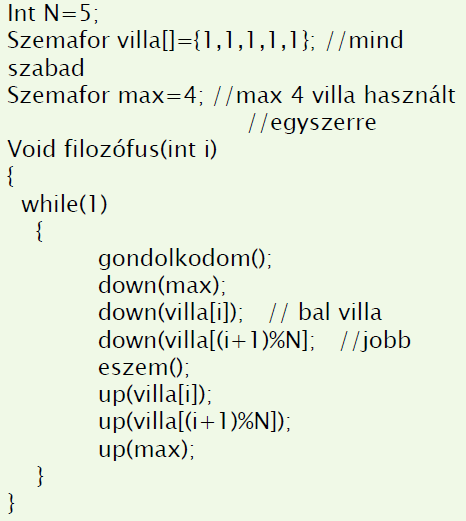
\includegraphics[width=0.3\textwidth]{img/filo.png}
              \caption{Étkező filozófusok, javított megoldás: 5 villa szemafor van, és egy maximum. Korlátozott erőforrás megszerzésre példa}
          \end{figure}
    \item Író-olvasó probléma: Adatbázist egyszerre többen olvashatják, de csak 1 folyamat írhatja.
          \begin{figure}[H]
              \centering
              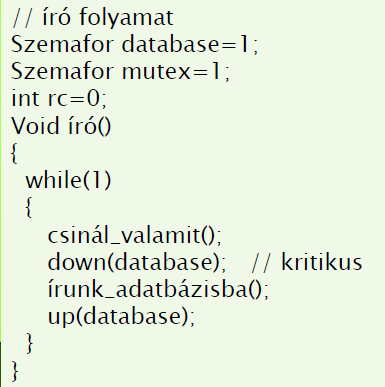
\includegraphics[width=0.3\textwidth]{img/iro.png}
              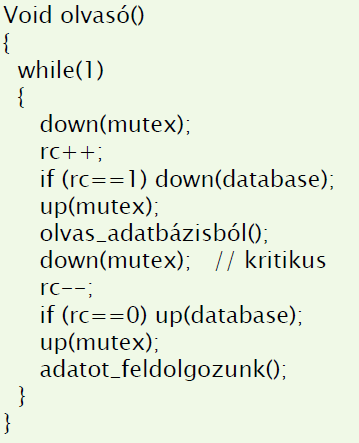
\includegraphics[width=0.3\textwidth]{img/olvaso.png}
              \caption{Író-olvasó probléma megvalósítása}
          \end{figure}
\end{itemize}

\section{Be- és kimeneti eszközök ütemezési lehetőségei, holtpontok}

\subsection{Be- és kimeneti eszközök ütemezési lehetőségei}

Input-Output eszközök:
\begin{itemize}
    \item \textit{Blokkos eszközök}. Adott méretű blokkban tároljuk az információt. Blokkméret 512 byte - 32768 byte között. Egymástól függetlenül írhatók vagy olvashatók. Blokkonként címezhetőek. Ilyen eszköz: HDD, szalagos egység
    \item \textbf{Karakteres eszközök}. Nem címezhető, csak jönnek-mennek sorban a
          ,,karakterek" (bájtok)
    \item \textbf{Időzítő}: kivétel, nem blokkos és nem
          karakteres
\end{itemize}
\textit{Megszakítások}: Általában az eszközöknek van állapotbitjük, jelezve, hogy az adat készen van. \\
Megszakítás használat (IRQ):
\begin{enumerate}
    \item CPU tevékenység megszakítása
    \item a kért sorszámú kiszolgáló végrehajtása
    \item a kívánt adat beolvasása, a szorosan hozzátartozó tevékenység elvégzése
    \item visszatérés a megszakítás előtti állapothoz.
\end{enumerate}
\textit{Közvetlen memória elérés}(DMA): Direct Memory Access, tartalmaz memória cím regisztert, átvitel irány jelzésre, mennyiségre regisztert. Ezeket szabályos in, out portokon lehet elérni. \\
Működés lépései:
\begin{enumerate}
    \item CPU beállítja a DMA vezérlőt. (Regisztereket.)
    \item A DMA a lemezvezérlőt kéri a megadott műveletre.
    \item Miután a lemezvezérlő beolvasta a pufferébe, a rendszersínen keresztül a memóriába(ból) írja, olvassa az adatot.
    \item Lemezvezérlő nyugtázza, hogy kész a kérés teljesítése.
    \item DMA megszakítással jelzi, befejezte a műveletet.
\end{enumerate}

\subsection{Holtpontok (deadlock)}

Két vagy több folyamat egy erőforrás megszerzése során olyan helyzetbe kerül, hogy egymást blokkolják a további végrehajtásban. Pontos definíció: Folyamatokból álló halmaz holtpontban van, ha minden folyamat olyan eseményre vár, amit csak a halmaz egy másik folyamata okozhat. Nem csak az I/O eszközökhöz kötődik, pl párhuzamos rendszerek, adatbázisok, stb. \\
Coffman E.G. szerint 4 feltétel szükséges a holtpont kialakulásához:
\begin{enumerate}
    \item \textit{Kölcsönös kizárás feltétel.} Minden erőforrás hozzá van rendelve 1 folyamathoz vagy szabad.
    \item \textit{Birtoklás és várakozás feltétel.} Korábban kapott erőforrást birtokló folyamat kérhet újabbat.
    \item \textit{Megszakíthatatlanság feltétel.} Nem lehet egy folyamattól elvenni az erőforrást, csak a folyamat engedheti el.
    \item \textit{Ciklikus várakozás feltétel.} Két vagy több folyamatlánc kialakulása, amiben minden folyamat olyan erőforrásra vár, amit egy másik tart fogva.
\end{enumerate}
Irányított gráffal lehet modellezni a folyamatokat és erőforrásokat. Ha van kör, akkor az holtpontot jelent. \\ \\
Stratégiék holtpont esetén:
\begin{enumerate}
    \item A probléma figyelmen kívül hagyása.
          \begin{itemize}
              \item Nem törődünk vele, nagy valószínűséggel Ő sem talál meg bennünket.
              \item Ezt a módszert gyakran strucc algoritmus néven is ismerjük.
              \item Vizsgálatok szerint a holtpont probléma és az egyéb (fordító, op.rendszer, hw, sw hiba) összeomlások aránya 1:250.
              \item A Unix, Windows világ is ezt a „módszert”	használja. De túl nagy az ár a várható haszonért cserébe.
          \end{itemize}
    \item Felismerés és helyreállítás.
          \begin{itemize}
              \item Engedjük a holtpontot megjelenni (kör), ezt észrevesszük és cselekszünk.
              \item Folyamatosan figyeljük az erőforrás igényeket, elengedéseket.
              \item Kezeljük az erőforrás gráfot folyamatosan. Ha kör keletkezik, akkor egy körbeli folyamatot megszüntetünk.
              \item Másik módszer, nem foglalkozunk az erőforrás gráffal, ha x (fél óra?) ideje 	blokkolt egy folyamat, egyszerűen megszüntetjük. Ez nagygépes rendszereknél ismert módszer.
          \end{itemize}
    \item Megelőzés.
          \begin{itemize}
              \item A 4 szükséges feltétel egyikének meghiúsítása.
              \item A Coffman féle 4 feltétel valamelyikére mindig él egy megszorítás.
                    \begin{itemize}
                        \item Kölcsönös kizárás. Ha egyetlen erőforrás soha nincs kizárólag 1 folyamathoz rendelve, akkor nincs holtpont se. De ez nehézkes, míg pl. nyomtató használatnál a
                              nyomtató démon megoldja a problémát, de ugyanitt a nyomtató puffer egy lemezterület, itt már kialakulhat holtpont.
                        \item Ha nem lehet olyan helyzet, hogy erőforrásokat birtokló folyamat további erőforrásra várjon, akkor szintén nincs holtpont. Ezt kétféle módon érhetjük el: Előre kell tudni egy folyamat összes erőforrásigényét vagy ha erőforrást akar egy folyamat, először engedje el az összes birtokoltat.
                        \item A Coffman féle harmadik feltétel a megszakíthatatlanság. Ennek elkerülése eléggé
                              nehéz. Pl nyomtatás közben nem szerencsés a nyomtatót másnak adni.
                        \item A negyedik feltétel, a ciklikus várakozás már könnyebben megszüntethető. Egyszerű mód: Minden folyamat egyszerre csak 1 erőforrást birtokolhat. Másik módszer: Sorszámozzuk az erőforrásokat, és a folyamatok csak ezen sorrendben kérhetik az erőforrásokat. Ez jó elkerülési mód, csak megfelelő sorrend nincs.
                    \end{itemize}
          \end{itemize}
    \item Dinamikus elkerülés.
          \begin{itemize}
              \item Erőforrások foglalása csak ,,óvatosan".
              \item Bankár algoritmus (Dijkstra, 1965) Mint a kisvárosi bankár hitelezési gyakorlata. A bankár algoritmus minden kérés megjelenésekor azt nézi, hogy a kérés teljesítése biztonságos
                    állapothoz vezet-e. Ha igen, jóváhagyja, ha nem, a kérést elhalasztja. Eredetileg 1 erőforrásra tervezett. \\
                    A korábbi megelőzés is, meg ez az elkerülés is olyan információt kér (az erőforrás pontos igényeket, a folyamatok számát előre), ami nehezen megadható. (Folyamatok dinamikusan jönnek létre, erőforrások dinamikusan módosulnak.) Ezért a gyakorlatban kevesen alkalmazzák.
              \item Biztonságos állapotok, olyan helyzetek, melyekből létezik olyan kezdődő állapotsorozat, melynek eredményeként mindegyik folyamat megkapja a kívánt erőforrásokat és befejeződik.
          \end{itemize}
\end{enumerate}

\section{Memóriakezelés, virtuális memória fogalma}

\textit{Monoprogramozás}: A legegyszerűbb memóriakezelési módszer, időben csak egyetlen programot futtatunk. \\
\textit{Multiprogramozás}: multiprogramozás rögzített partíciókkal: Ekkor a rendelkezésre álló memóriát felosztják több, általában nem egyforma hosszúságú részre. Működéséhez minden partíciónak szüksége van egy úgynevezett várakozási sorra. Ha beérkezik egy igény, az operációs rendszer berakja annak a legkisebb méretű, partíciónak nevezett rész várakozási sorába, ahová még befér. Ilyenkor elvész a partíciónak az a része – nem használható –, amit az éppen futó processz nem használ. Ha az adott szeletben befejeződik a munka, a legrégebben várakozó megkapja a területet, és elkezd működni.

\subsection{Memóriakezelés}

A memóriakezelő az operációs rendszer része, gyakran a kernelben. Feladata: a memória nyilvántartása, melyek szabadok, foglaltak; memóriát foglaljon folyamatok számára; memóriát felszabadítson; csere vezérlése a RAM és a (Merev)Lemez között. \\
Kétféle algoritmus csoport:
\begin{itemize}
    \item Szükséges a folyamatok mozgatása, cseréje a memória és a lemez között. (swap)
    \item Nincs erre szükség, ha elegendő memória van.
\end{itemize}

\textit{Multiprogramozás rögzített memóriaszeletekkel}: Osszuk fel a memóriát n (nem egyenlő) szeletre. (Fix szeletek) Pl. rendszerindításnál ez megtehető. Egy közös várakozási sor van, minden szeletre külön-külön várakozási sor. Kötegelt rendszerek tipikus megoldása. \\
\textit{Relokáció}: Nem tudjuk hova kerül egy folyamat, így a memória hivatkozások nem fordíthatók fix értékekre. \\
\textit{Védelem}: Nem kívánatos, ha egy program a másik memóriáját ,,éri el". \\
Másik megoldás: Bázis+határregiszter használata, ezeket a programok nem módosíthatják, de minden címhivatkozásnál ellenőrzés: lassú. \\
\textit{Multiprogramozás memóriacsere használattal}: A korábbi kötegelt rendszerek tipikus megoldása a	rögzített memória szeletek használata (IBM OS/MFT). Időosztásos, grafikus felületek esetén ez nem az igazi. Itt a teljes folyamatot mozgatjuk a memória-lemez között. Nincs rögzített memória partíció, mindegyik	dinamikusan változik, ahogy az op. rendszer oda-vissza rakosgatja a folyamatokat. Dinamikus, jobb memória kihasználtságú lesz a rendszer, de a sok csere lyukakat hoz létre, ezért memória tömörítést kell végezni. (Sok esetben ez az időveszteség nem megengedhető.) \\
\textit{Dinamikus memóriafoglalás}: Általában nem ismert, hogy egy programnak mennyi dinamikus adatra, veremterületre van szüksége. A program ,,kód" része fix szeletet kap, míg az adat és verem része változót. Ezek tudnak nőni (csökkenni). Ha elfogy a memória, akkor a folyamat leáll, vár a
folytatásra, vagy kikerül a lemezre, hogy a többi még futó folyamat memóriához jusson. Ha van a memóriában már várakozó folyamat, az is cserére kerülhet. \\
A ,,dinamikus" memória nyilvántartása:
\begin{itemize}
    \item Allokációs egység definiálása. Ennek mérete kérdés. Ha kicsi, akkor kevésbé lyukasodik a memória, viszont nagy a nyilvántartási ,,erőforrás (memória) igény". Ha nagy az egység, akkor túl sok lesz az egységen belüli maradékokból adódó memóriaveszteség.
    \item A nyilvántartás megvalósítása: Bittérkép használattal vagy Láncolt lista használattal. Ha egy folyamat befejeződik, akkor szükség lehet az egymás melletti memória lyukak egyesítésére. Külön lista a lyukak és folyamatok listája.
\end{itemize}
\textit{Memóriafoglalási stratégiák}: Új vagy swap partícióról behozott folyamat számára, több memória elhelyezési	algoritmus ismert (hasonlóak a lemezhez):
\begin{itemize}
    \item First Fit (első helyre, ahova befér, leggyorsabb, legegyszerűbb)
    \item Next Fit (nem az elejéről, hanem az előző befejezési pontjából indul a keresés, kevésbé hatékony, mint a first fit)
    \item Best Fit (lassú, sok kis lyukat produkál)
    \item Worst Fit (nem lesz sok kis lyuk, de nem hatékony)
    \item Quick Fit (méretek szerinti lyuklista, a lyukak összevonása költséges)
\end{itemize}

\subsection{Virtuális memória fogalma}

\textit{Multiprogramozás virtuális memóriahasználattal}: Egy program használhat több memóriát,
mint a rendelkezésre álló fizikai méret. Az operációs rendszer csak a ,,szükséges részt" tartja a fizikai memóriában. Egy program a ,,virtuálismemória-térben" tartózkodik. Az elv akár a monoprogramozás környezetben is használható. \\
\textit{Memory Management Unit (MMU)}: A virtuális címtér ,,lapokra" van osztva. (Ezt laptáblának
nevezzük). Van jelenlét/hiány bit. Virtuális-fizikai lapokat összerendeljük. Ha az MMU látja, hogy egy lap nincs a memóriában, laphibát okoz, op.rendszer kitesz egy lapkeretet, majd behozza a szükséges lapot.

\section{Lapozás és szegmentálás}

\subsection{Lapozás}

\textit{Lapozástervezési szempontok}:
\begin{itemize}
    \item Munkahalmaz modell
          \begin{itemize}
              \item A szükséges lapok betöltése. (Induláskor-előlapozás) A folyamat azon lapjainak fizikai memóriában tartása, melyeket használ. Ez az idővel változik.
              \item Nyilván kell tartani a lapokat. Ha egy lapra az utolsó N időegységben nem hivatkoznak, laphiba esetén kidobjuk.
              \item Óra algoritmus javítása: Vizsgáljuk meg, hogy a lap eleme a munkahalmaznak? (WSClock algoritmus)
          \end{itemize}
    \item Lokális, globális helyfoglalás
          \begin{itemize}
              \item Egy laphibánál ha az összes folyamatot (globális), vagy csak a folyamathoz tartozó (lokális) lapokat vizsgáljuk.
              \item Globális algoritmus esetén minden folyamatot elláthatunk méretéhez megfelelő lappal, amit aztán dinamikusan változtatunk.
              \item Page Fault Frequency (PFF) algoritmus, laphiba/másodperc arány, ha sok a laphiba, növeljük a folyamat memóriában lévő lapjainak a számát. Ha sok a folyamat, akár teljes folyamatot lemezre vihetünk.(teherelosztás)
          \end{itemize}
    \item Helyes lapméret meghatározása.
          \begin{itemize}
              \item Kicsi lapméret: A ,,lapveszteség" kicsi, viszont nagy laptábla kell a nyilvántartáshoz.
              \item Nagy lapméret: Fordítva, ,,lapveszteség" nagy, kicsi laptábla.
              \item Jellemzően: n x 512 bájt a lapméret, XP, Linuxok 4KB a lapméret. 8KB is használt (szerverek).
          \end{itemize}
    \item Közös memória
          \begin{itemize}
              \item Foglalhatunk memóriaterületet, amit több folyamat használhat.
              \item Elosztott közös memória: Hálózatban futó folyamatok közti memóriamegosztás.
          \end{itemize}
\end{itemize}

\subsection{Szegmentálás}

Virtuális memória: egy dimenziós címtér, 0-tól a maximum címig (4,8,16 GB, ...). \\
Több programnak van dinamikus területe, melyek növekedhetnek, bizonytalan mérettel. Hozzunk létre egymástól független címtereket, ezeket szegmensnek nevezzük. \\
Ebben a világban egy cím 2 részből áll: szegmens szám, és ezen belüli cím. (eltolás) \\
Szegmentálás lehetővé teszi osztott könyvtárak ,,egyszerű" megvalósítását. Logikailag szét lehet szedni a programot, adat szegmens, kód szegmens stb. Védelmi szintet is megadhatunk egy szegmensre. Lapok fix méretűek, a szegmensek nem. Szegmens töredezettség megjelenése. Ez töredezettség-összevonással javítható.

\section{Lapcserélési algoritmusok}

Ha nincs egy virtuális című lap a memóriában, akkor egy lapot ki kell dobni, berakni ezt az új lapot. A processzor gyorsító tár (cache) memória használatnál, vagy a böngésző helyi gyorsítótáránál is hasonló a helyzet.
Optimális lapcserélés: Címkézzünk meg minden lapot azzal a számmal, ahány CPU utasítás végrehajtódik, mielőtt hivatkozunk rá. Dobjuk ki azt a lapot, amelyikben legkisebb ez a szám. Egy baj van, nem lehet megvalósítani, viszont kétszeres futásnál tesztelési célokat szolgálhat.
\begin{itemize}
    \item NRU (Not Recently Used) algoritmus:
          \begin{itemize}
              \item Használjuk a laptábla bejegyzés módosítás (Modify) és hivatkozás (Reference) bitjét. A hivatkozás bitet időnként (óramegszakításnál, kb. 0.02 sec) állítsuk 0-ra, ezzel azt jelezzük, hogy az ,,utóbbi időben" volt-e használva, hivatkozva.
                    \begin{itemize}
                        \item 0.osztály: nem hivatkozott, nem módosított
                        \item 1.osztály: nem hivatkozott, módosított. Ide akkor lehet kerülni, ha az óramegszakítás állítja 0-ra a hivatkozás bitet.
                        \item 2.osztály: hivatkozott, nem módosított
                        \item 3.osztály: hivatkozott, módosított
                    \end{itemize}
              \item Válasszunk véletlenszerűen egy lapot a legkisebb nem üres osztályból. Egyszerű, nem igazán hatékony implementálni, megfelelő eredményt ad.
          \end{itemize}
    \item FIFO lapcserélés. Egyszerű FIFO, más területekről is ismert, ha szükség van egy új lapra akkor a legrégebbi lapot dobjuk ki. Listában az érkezés sorrendjében a lapok, egy lap a lista elejére érkezik, és a végéről távozik. Ennek javítása a Második Lehetőség lapcserélő algoritmus.
    \item Második Lehetőség lapcserélő algoritmus. Olyan, mint a FIFO, csak ha a lista végén lévő lapnak a hivatkozás bitje 1, akkor kap egy második esélyt, a lista elejére kerül és a hivatkozás bitet 0-ra állítjuk.
    \item Óra algoritmus: olyan, mint a második lehetőség, csak ne a lapokat mozgassuk körbe egy
          listában, hanem rakjuk körbe őket és egy mutatóval körbe járunk. A mutató a legrégebbi lapra mutat. Laphibánál, ha a mutatott lap hivatkozás bitje 1, nullázzuk azt, és a következő lapot
          vizsgáljuk. Ha vizsgált lap hivatkozás bitje 0, akkor kitesszük.
    \item LRU (Least Recently Used) algoritmus: Legkevésbé (legrégebben) használt lap kidobása. HW vagy SW megvalósítás.
          \begin{itemize}
              \item HW1: Vegyünk egy számlálót, ami minden memória hivatkozásnál 1-gyel nő. Minden laptáblában tudjuk ezt a számlálót tárolni. Minden memóriahivatkozásnál ezt a számlálót beírjuk a lapba. Laphibánál megkeressük a legkisebb számlálóértékű lapot.
              \item HW2: LRU bitmátrix használattal, n lap, n x n bitmátrix. Egy k. lapkeret hivatkozásnál állítsuk a mátrix k. sorát 1-re, míg a k. oszlopát 0-ra. Laphibánál a legkisebb értékű sor a legrégebbi.
          \end{itemize}
    \item NFU (Not Frequently Used) algoritmus:
          \begin{itemize}
              \item Minden laphoz tegyünk egy számlálót. Minden óramegszakításnál ehhez adjuk hozzá a lap
                    hivatkozás (R) bitjét.
              \item Laphibánál a legkisebb számlálóértékű lapot dobjuk ki. (A leginkább nem használt lap)
              \item Hiba, hogy az NFU nem felejt, egy program elején gyakran használt lapok megőrzik nagy értéküket.
              \item Módosítsuk: Minden óramegszakításnál csináljunk jobbra egy biteltolást a számlálón, balról pedig hivatkozás bitet tegyük be (shr).(Öregítő algoritmus)
              \item Ez jól közelíti az LRU algoritmust.
              \item Ez a lapszámláló véges bitszámú (n), így n időegység előtti eseményeket biztosan nem tud megkülönböztetni.
          \end{itemize}
\end{itemize}

\section{Lemezterület-szervezés, redundáns tömbök, fájlrendszerek szolgáltatásai és jellemző megvalósításaik}

\subsection{Lemezterület-szervezés}

\subsection{Redundáns tömbök}

RAID -- Redundant Array of Inexpensive Disks. Ha operációs rendszer nyújtja, gyakran Soft Raidnek nevezik. Ha intelligens (külső) vezérlőegység nyújtja, gyakran Hardver Raid-nek, vagy csak Raid diszkrendszernek nevezik. Bár nevében olcsó (Inexpensive), valójában inkább nem az. Több lemezt fog össze, és egy logikai egységként látja az operációs rendszer. Többféle ,,összefogási" elv létezik: RAID 0-6.
\begin{itemize}
    \item RAID 0(striping)
          \begin{itemize}
              \item Ez az a Raid, ami nem is redundáns
              \item Több lemez logikai összefűzésével egy meghajtót kapunk.
              \item A lemezkapacitások összege adja az új meghajtó kapacitását.
              \item A logikai meghajtó blokkjait szétrakja a lemezekre (striping), ezáltal egy fájl írása több lemezre kerül.
              \item Gyorsabb I/O műveletek.
              \item Nincs meghibásodás elleni védelem.
          \end{itemize}
    \item RAID 1(tükrözés)
          \begin{itemize}
              \item Két független lemezből készít egy logikai egységet.
              \item Minden adatot párhuzamosan kiír mindkét lemezre.(Tükrözés, mirror)
              \item Tárolókapacitás felére csökken.
              \item Drága megoldás.
              \item Jelentős hibatűrő képesség. Mindkét lemez egyszerre történő meghibásodása okoz adatvesztést.
          \end{itemize}
    \item RAID 1+0, RAID 0+1
          \begin{itemize}
              \item RAID 1+0: Tükrös diszkekből vonjunk össze többet.
              \item RAID 0+1: RAID 0 összevont lemezcsoportból vegyünk kettőt.
              \item A vezérlők gyakran nyújtják egyiket, másikat, mivel így is, úgy is tükrözés van, azaz drága, így ritkán használt.
          \end{itemize}
    \item RAID 2: Adatbitek mellett hibajavító biteket is tartalmaz. (ECC: Error Correction Code) Pl. 4 diszkhez 3 javító diszk
    \item RAID 3: Elég egy plusz ,,paritásdiszk", n+1 diszk, $\sum{n}$ a kapacitás
    \item RAID 4: RAID 0 kiegészítése paritásdiszkkel.
    \item Ma ezen megoldások (RAID 2,3,4) nem gyakran használatosak.
    \item RAID 5
          \begin{itemize}
              \item Nincs paritásdiszk, ez el van osztva a tömb összes elemére. (stripe set)
              \item Adatok is elosztva kerülnek tárolásra.
              \item Intenzív CPU igény (vezérlő CPU!!!)
              \item Redundáns tárolás, 1 lemez meghibásodása nem okoz adatvesztést. A paritásbitből meg a többiből az egy eltűnt kiszámítható. 2 lemez egyidejű meghibásodása már okoz adatvesztést.
              \item N lemez RAID 5 tömbben (N>=3), n-1 lemez méretű logikai meghajtót ad.
          \end{itemize}
    \item RAID 6
          \begin{itemize}
              \item A RAID 5 paritásblokkhoz, hibajavító kód kerül tárolásra.(+1 diszk)
              \item Még intenzívebb CPU igény.
              \item Két diszk egyidejű kiesése sem okoz adatvesztést.
              \item Relatív drága
              \item N diszk RAID 6-os tömbjének kapacitása, N-2 diszk kapacitással azonos.
              \item Elvileg általánosítható a módszer (3 diszk kiesése)
          \end{itemize}
\end{itemize}
Ma leggyakrabban a RAID 1,5 verziókat használják. A RAID 6 vezérlők az utóbbi 1-2 évben jelentek meg. Bár olcsó diszkekről szól a RAID, de valójában ezek nem mindig olcsók. RAID 6-nl már 2 lemez kiesik, így ez még inkább drága. \\
Hot-Swap(forró csere) RAID vezérlő: működés közben a meghibásodott lemezt egyszerűen kicseréljük.

\subsection{Fájlrendszerek szolgáltatásai}

\textit{Fájl}: adatok egy logikai csoportja, névvel egyéb paraméterekkel ellátva. A fájl az információtárolás egysége, névvel hivatkozunk rá. Jellemzően egy lemezen helyezkedik el, de általánosan az adathalmaz, adatfolyam akár képernyőhöz, billentyűzethez is köthető. \\
A lemezen általában 3 féle fájl, állomány található:
\begin{itemize}
    \item Rendes felhasználói állomány.
    \item Ideiglenes állomány
    \item Adminisztratív állomány. Ez a működéshez szükséges, általában rejtett.
\end{itemize}
\textit{Könyvtár}: fájlok (könyvtárak) logikai csoportosítása. \\
\textit{Fájlrendszer}: módszer, a fizikai lemezünkön, kötetünkön a fájlok és könyvtárak elhelyezés rendszerének kialakítására. \\
Fájlok elhelyezése: A partíció elején, az ún. Szuperblokk (pl. FAT esetén a 0. blokk ) leírja a rendszer jellemzőit. Általában következik a helynyilvántartás (FAT, láncolt listás nyilvántartás). Ezután a könyvtárszerkezet (inode), a könyvtár bejegyzésekkel, fájl adatokkal. (FAT16-nál a könyvtár előbb van, majd utána a fájl adatok.) \\
Elhelyezési stratégiák:
\begin{itemize}
    \item Folytonos tárkiosztás: First Fit, Best Fit, Worst Fit (olyan memória szakaszba tesszük, hogy a lehető legnagyobb rész maradjon szabadon). Veszteséges lemezkihasználás.
    \item Láncolt elhelyezkedés: Nincs veszteség (csak a blokkméretből adódóan). Fájl adatok (blokkokra bontva) láncolt lista tábla. Az n. blokk olvasása lassú lesz. Szabad-foglalt szektorok: File Allocation Table,FAT. Ez nagy lehet, a FAT-nak a memóriában kell lenni fájl műveletnél.
    \item Indextáblás elhelyezés: Katalógus tartalmazza a fájlhoz tartozó kis tábla (inode) címét. Egy inode címből elérhető a fájl.
\end{itemize}

Fájlrendszer típusok:
\begin{itemize}
    \item Merevlemezen alkalmazott fájlrendszer: FAT, NTFS, EXT2FS, XFS, stb
    \item Szalagos rendszereken (elsősorban backup) alkalmazott fájlrendszer: Tartalomjegyzék, majd a tartalom szekvenciálisan
    \item CD, DVD, Magneto-opto Disc fájlrendszer: CDFS, UDF (Universal Disc Format), kompatibilitás
    \item RAM lemezek (ma már kevésbé használtak)
    \item FLASH memória meghajtó (FAT32)
    \item Hálózati meghajtó: NFS
    \item Egyéb pszeudó fájlrendszerek: Zip, tar.gz, ISO
\end{itemize}

\textit{Naplózott fájlrendszerek}: A fájlrendszer sérülés, áramszünet stb. esetén inkonzisztens állapotba kerülhet. Gyakran nevezik: LFS-nek (Log-structured File System) vagy JFS-nek(Journaled). Adatbázis-kezelők mintájára: művelet + log naplózódik. Tranzakciós alapra épül. Leállás, hiba esetén a log alapján helyre lehet állítani. Célszerűen a log másik lemez (másik partíció). Nagyobb erőforrás igényű, de nagyobb a megbízhatóság. \\
A mai operációs rendszerek ,,rengeteg" típust támogatnak, pl: Linux 2.6 kernel több mint 50-et.
A fájlrendszert csatolni többféleképpen is lehet:
\begin{itemize}
    \item Mount, eredményeképpen a fájlrendszer állományok elérhetők lesznek.
    \item Automatikus csatolás (pl. USB drive)
    \item Kézi csatolás (Linux, mount parancs)
\end{itemize}
Külön névtérbeli elérhetőség a Windowsnál az A, B, C stb lemezek. Egységes névtér a UNIX-nál van.

\subsection{Fájlrendszerek szolgáltatásainak jellemző megvalósításai}

\begin{itemize}
    \item FAT
          \begin{itemize}
              \item File Allocation Table. Talán a legrégebbi, ma is élő fájlrendszer.
              \item A FAT tábla a lemez foglaltsági térképe, annyi eleme van, ahány blokk a lemezen. Pl: Fat12, FDD, Cluster méret 12 bites. Ha értéke 0, szabad, ha nem, foglalt. Biztonság kedvéért 2 tábla van.
              \item Láncolt elhelyezés. A katalógusban a file adatok (név stb) mellett csak az első fájl blokk sorszáma van megadva. A FAT blokk azonosító mutatja a következő blokk címét. Ha nincs tovább, FFF az érték.
              \item Rögzített bejegyzés méret, 32 bájt (max. 8.3 név)
              \item System, Hidden, Archive, Read only, könyvtár attribútumok
              \item A fájl utolsó módosítás ideje is tárolva van.
              \item \textit{FAT16}, 16 bites cluster leíró, 4 bájt (2x2) írja le a fájl kezdőblokkját. Max. 4 GB partíciós méret (64kb blokk méretnél), jellemzően 2 GB. Fájlméret maximum is a 4 (2) GB. Külön könyvtári terület (FDD-nez a 0. sáv). FDD-n 512 könyvtári bejegyzés. HDD-n 32736 könyvtári bejegyzés (16 bit előjelesen)
              \item \textit{FAT32} (1996-tól elérhető): 28 bites clusterleíró, 2 TB partíciós méret (alap szektor mérettel), 32 MB-ig 1 blokk = 1 szektor(512bájt). 64 MB: 1 blokk=1KB (2 szektor), 128MB: 1 blokk=2KB. 1 blokk max. 64 KB lehet.
              \item Támogatták már a hosszú fájl neveket is. Többszörös 8.3 részre fenntartott bejegyzésekkel.
              \item Töredezettségmentesítés szükséges.
          \end{itemize}
    \item NTFS
          \begin{itemize}
              \item New Technology File System
              \item FAT-NTFS hatékonysági határ: kb. 400 MB.
              \item 255 karakteres fájl név, 8+3 másodlagos név
              \item Kifinomult biztonsági beállítások
              \item Ahogy a FAT esetén, itt is szükséges a töredezettségmentesítés.
              \item Titkosított fájlrendszer támogatása, naplózás
              \item POSIX támogatás. Hardlink (fsutil parancs), időbélyegek, kis-nagybetűk különböznek
              \item Tömörített fájl, mappa, felhasználói kvóta kezelés
              \item Az NTFS csak klasztereket tart nyilván, szektort (512bájt) nem

                    \begin{figure}[H]
                        \centering
                        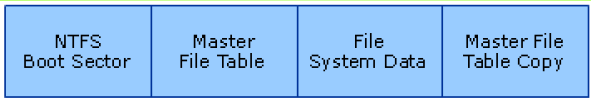
\includegraphics[width=0.9\textwidth]{img/ntfs.png}
                        \caption{NTFS partíció. A Master File Table és a File System Data egy-egy táblázat}
                    \end{figure}

              \item MFT: NTFS partíció az MFT (Master File Table) táblázattal kezdődik. 16 attribútum ad egy fájl bejegyzést. Minden attribútum max. 1kb. Ha ez nem elég, akkor egy attribútum mutat a folytatásra. Az adat is egyfajta attribútum, így egy bejegyzés több adatsort tartalmazhat. (PL: Betekintő kép) Elvi fájlméret $2^64$ bájt lehet. Ha a fájl < 1kb, belefér az attribútumba, közvetlen fájl. Nincs fájlméret maximum.
          \end{itemize}
          \begin{figure}[H]
              \centering
              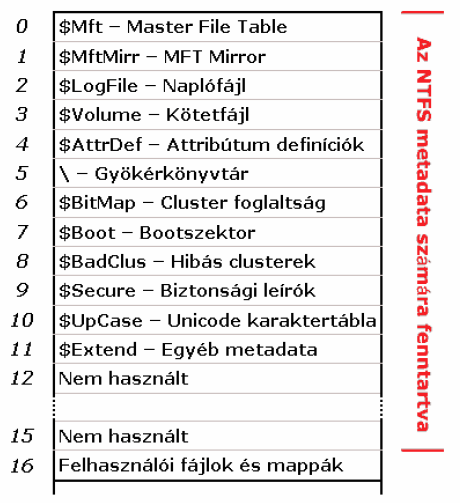
\includegraphics[width=0.6\textwidth]{img/ntfs2.png}
              \caption{Az NTFS partíció felépítése}
          \end{figure}
    \item ext, az ext2 és az ext3
          \begin{itemize}
              \item Az „ext” kifejezés a fájlrendszerek neveiben az extended (magyarul kiterjesztett) kifejezést takarja. Az extended fájlrendszer volt az első kifejezetten a UNIX-szerű GNU/LINUX operációs rendszerekhez készített fájlrendszer, amely örökölte az UFS (UNIX File System) fájlrendszer metaadat-szerkezetét, és arra készült, hogy a Minix operációs rendszer fájlrendszerének a hibáit kiküszöbölje. A hibák kiküszöbölése többek között a Minix operációs rendszer fájlrendszer-határainak kiterjesztése.
              \item Az ext2 fájlrendszer, amely a GNU/LINUX operációs rendszereken kívül más rendszereken is megjelent, több Linux disztribúció alapértelmezett fájlrendszere volt, amíg az utódja, az „ext3” fájlrendszer (third extended filesystem – harmadik kiterjesztett fájlrendszer) el nem készült.
              \item Az ext3 fájlrendszer (third extended filesystem – harmadik kiterjesztett fájlrendszer) az ext2 fájlrendszer utódja, amely már az ext2 fájlrendszerhez képest naplózást is tartalmaz. Ez a naplózás elsősorban a biztonságot növeli, és lehetővé teszi azt, hogy szabálytalan leállás bekövetkezése után ne kelljen az egész fájlrendszert újra ellenőrizni.
          \end{itemize}
    \item ReiserFS: A ReiserFS fájlrendszer lehetővé teszi egy blokkos eszközön (block device) változó méretű fájlok tárolását és könyvtárstruktúrába rendezését. A kezdeti UNIX és UNIX-szerű operációs rendszerek (így pl. a GNU/LINUX operációs rendszer is) csak egyfajta fájlrendszert támogattak, a saját formátumukat. A modern operációs rendszerek viszont többféle fájlrendszert is támogatnak, és vannak olyan fájlrendszerek is, amelyeket több operációs rendszer is támogat. A ReiserFS fájlrendszer egyáltalán nem ilyen. A ReiserFS fájlrendszer egy olyan fájlrendszer, amely csak és kizárólag a GNU/LINUX operációs rendszer alatt használható jelenleg korlátozás nélkül.
\end{itemize}

\end{document}